\chapter{Shell脚本基础}\label{chap:Shell脚本基础}
\minitoc

% 请在下方的大括号相应位置填写正确的节标题和标签,以及作者姓名
\section{第一个脚本}\label{sec:第一个脚本}
\sectionAuthor{Jiaqi Z.}

\begin{Abstract}
    \item 什么是Shell脚本
    \item 如何编写第一个Shell脚本——Hello World
    \item 如何运行脚本
\end{Abstract}

在前面的学习中,我们已经了解如何使用Linux命令在Shell进行操作,我们了解了如何对文件和目录进行简单的操作(如删除、复制等),同时我们也了解了一些更复杂的操作,例如使用\code{grep}和\code{sed}进行文本的查找和替换等。最后,我们还了解了如何使用\code{for}循环来进行批量操作。

而在一些特殊的场景下,我们可能希望做更复杂的操作,或者说,我们希望更简单地执行一些操作(这两句话本质上是一样的)。例如,如果我们每次都需要使用\code{sed}命令修改特定的内容,如\code{ENCUT = 400},刚开始还好,时间长了可能就会“嫌麻烦”。此时可能就会希望有一个单独的命令(比如叫做\code{changeENCUT})来实现这一功能。而实现这一功能的方法,就是使用\emph{脚本}。

在本章,我们将会讨论如何编写自己的脚本。类似于编程语言,脚本里面将会包含大量的编程思想——如输入、输出、条件、判断、函数等。在学习这一部分之前,希望你已经有了部分编程语言基础(没有也没有关系)。

\begin{extend}
    关于Shell和Bash的区别:一般来说,Shell指的是系统和用户交互的那层“外壳”,之前我们所学习的内容,其操作都是在Shell当中进行的。Shell具有多种版本,如“Bourne Shell”、“Bourne Again Shell”、“C Shell”等。其中,“Bourne Again Shell”就是我们所谓的“bash”。在你的操作系统下,可以使用\code{top}命令查看其Shell类型。
    
    Shell脚本,全称叫做“Shell Script”,是一种在Shell当中批量运行多条语句的程序。
    
    由于目前主流的Shell是基于Bash解释的,而我们所写的Shell脚本,实际上也大多都是Bash脚本,因此在后文当中,我们可能不会精确区分Bash脚本和Shell脚本的区别。
\end{extend}

\subsection{编写第一个脚本}\label{subsec:第一个脚本-编写第一个脚本}

正如任何程序的开始都是“Hello World”,在本章我们也不例外。在Linux当中编写Shell脚本不需要额外的程序,只需要使用\code{vi}编写一段文本文件,并\emph{赋予它运行权限},就可以作为脚本运行了。首先通过\code{vi}创建一个名为\code{hello}的文件,并输入如下内容:

\begin{lstlisting}[language=bash,label=hello]
#!/bin/bash
# 输出Hello World!
echo "Hello World!"
\end{lstlisting}

编写完成后保存,并添加运行权限(\code{chmod +x hello},详见第\ref{sec:文件权限管理}一节),然后执行\code{./hello},即可在屏幕上看到输出结果。

\begin{attention}
    在运行时需要加上\code{./}表示在当前目录寻找命令。在Linux当中,不添加\code{./}表示在环境变量\code{PATH}下查找文件运行,你可以在家目录下找到\code{.bashrc}的文件,里面包含有一系列配置Bash的命令,其中就有对环境变量的设置。

    在运行前,你需要保证程序已经具有运行权限,或者可以使用\code{source ./hello}或\code{. ./hello}的方式(二者等价)“临时赋予运行权限”\footnote{这是表面上的用法,事实上,\keyword{source}本意是\emph{在当前Shell下运行文件}。相对的,其他的用法(不加\code{source})则是在当前shell下新建了一个“子Shell”运行代码,其运行结果(例如一些变量)并不会带回外面。}。
\end{attention}

其中,代码第一行\code{\#!/bin/bash}表示\emph{使用bash运行}。正如前面所说的那样,Shell具有多种版本,因此,在编写时应当特别指定你所使用的版本。由于目前大多数Shell都是使用Bash,因此这一行在有些时候“可以省略”。但我们不建议将其省略,因为\emph{你永远不能保证你的这个脚本今后会在哪个版本的Shell下运行}。

\begin{extend}
    你可以想见,\code{/bin/bash}就是\code{bash}命令所在位置,你可以去看一下是不是真的存在。在查看的时候,注意是从“根目录”开始而不是“家目录”

    如果你真的这么做了,一种简单的方法是在\code{/bin/}目录下使用\code{ls | grep bash}只输出具有“bash”的文件,从而简化输出结果。当然,你也可以直接使用\code{ls bash}查看。

    当然,不建议你尝试使用\code{vi bash}查看里面的内容,\emph{它不是文本文件}。
\end{extend}

代码第二行以\code{\#}开头表示\emph{注释}。如同编写其他代码一样,使用注释是一个好习惯,它可以帮助你划分代码段落,以及记住对应的功能。随着学习的深入,我们会编写越来越长的脚本。因此,记得加注释是个好习惯。

第三行是这一脚本的关键,它使用\keyword{echo}实现字符串的输出。事实上,Shell脚本的每一个命令都可以在Shell本身下运行。因此,你也可以直接在Shell运行这一命令,会实现同样的效果。而编写脚本之后,就可以直接通过\code{./hello}实现这一功能,这便是脚本的作用。

\begin{attention}
    \code{echo}会将它后面的所有内容输出(在其他一些编程教材中,会将这一功能叫做“应声虫”,实际上,echo也就是“回音”的意思)。我们在这里添加双引号是为了强调它们是整体的,事实上,当你去掉这两个双引号,对程序运行结果没有任何影响。

    如果你在你的脚本中编写了代码,并同样使用了双引号,请注意:\emph{使用英文符号而不是中文符号},这一点在后续所有脚本编写过程中都应当注意。一般来说,我们不建议在脚本当中添加中文,虽然你写\code{echo "你好,世界!"}可能也会得到正确的结果,但不会永远如此。

    在本章的教程中,为了考虑到读者水平,我们的注释部分都会采用中文,如果这样也会引起脚本运行的失败(在测试时正常,但不敢保证在你的电脑也会正常),请删除中文注释后运行。
\end{attention}

\subsection{添加至环境变量}\label{subsec:第一个脚本-添加至环境变量}

正如前面所说,使用\code{./hello}表示在当前目录下查找名为\code{hello}的脚本并运行。这可以帮助我们快速调试代码,但在真正应用时,我们可能会希望在任何目录下运行脚本。此时就会希望将代码添加至环境变量,也就是前面所说的\code{PATH}。添加方法有两种——将脚本放置到已有的环境变量中,或者将脚本所在的目录设置为环境变量。

你可以通过\code{\$PATH}命令输出当前环境变量,通常来说,你可以将你所编写的脚本命令放置在\code{\texttilde/bin/}目录下(这一般都是用户的环境变量)完成后,你可以在任何目录下运行你的脚本了(不需要\code{./}了)。例如,在完成上述配置后,在任何目录下运行只需要使用\code{hello}即可。

如果你编写了一系列脚本,一个简单的方法是直接将它们所在的目录设置成“环境变量”。此时需要通过\code{.bashrc}文件。假设你的脚本所在目录为\code{\texttilde/bash/},使用\code{vi}打开\code{.bashrc}文件,在最后一行添加\code{export PATH=\$HOME/bash:\$PATH}即可。

其中,\keyword{export}是用来设置“环境变量”的命令,后面的\code{PATH=...}则是“变量赋值”的过程(后面就会学到)。\code{\$HOME}是系统内置的变量,表示\emph{用户的家目录},你可以在Shell下使用\code{echo \$HOME}查看变量的值\footnote{在这里我们又不知不觉接触到\code{echo}的新用法:输出变量的值。这本是后面的内容,在这里你可以提前先了解一下。},后面的\code{\$PATH}则表示原先的环境变量。

简单说,这一语句的意思就是在原有的\code{PATH}变量前面添加一个新的\code{\$HOME/bash}。添加完成后你需要使用\code{source \texttilde/.bashrc}命令“激活”这一环境变量(或者重启也可以实现这一功能),然后即可在任何地方如一般运行命令一样运行你在\code{\texttilde/bash/}目录下所有的脚本了。

\begin{attention}
    在后面的教学演示中,我们都不会添加\code{./}运行脚本(或者说,只有在这一节我们会详细提到如何运行脚本,后面都简单说作“运行脚本”)。如无特殊说明,无论是哪种方法(在当前目录、添加环境变量),运行最终效果都是一样的,后面不再赘述。

    为了你的方便,建议新建一个目录作为你后续练习脚本的目录,并使用上面的方法将其添加到环境变量中。
\end{attention}


\subsection{错误处理}\label{subsec:第一个脚本-错误处理}

\subsubsection{-bash: <脚本名>: Permission denied}

这可能是因为你在运行脚本时没有赋予其运行权限而直接运行脚本,如果你没有赋予权限,请使用\code{source}命令或\code{.}运行脚本。这同样适用于环境变量中的命令。对于环境变量中没有运行权限的脚本,需要使用\code{source <脚本名>}或\code{. <脚本名>}执行。
% 请在下方的大括号相应位置填写正确的节标题和标签,以及作者姓名
\section{变量}\label{sec:变量}
\sectionAuthor{Jiaqi Z.}

% 请在下方的item内填写本节知识点
\begin{Abstract}
    \item 如何在脚本中定义变量
    \item 如何输出变量
    \item 如何对变量进行简单运算
\end{Abstract}

% 请在正文相应位置填写正确的小节标题(或小小节标题),同时将标签的“节标题”和“小节标题”改为实际内容

如果所有脚本都只能按照固定的内容运行,显然功能太弱了。与其他编程语言类似,脚本语言应当也具有类似于“\emph{变量}”的功能实现“可拓展性”。

所谓“变量”,指的就是\emph{在运行过程中会发生变化的量},这些值可能是由用户输入给定的,或者在运行过程中生成的,或者是通过文件读取得到的。

\subsection{定义变量与初始化}\label{subsec:变量-定义变量与初始化}

与C语言等强类型语言不同,Shell脚本的变量在使用之前不需要对其进行“声明”,相对地则是需要对其进行\emph{初始化}。与其他编程语言类似,在Shell脚本中,第一次使用变量时需要对变量进行赋值(也可以叫做“初始化”)。例如,我们希望将字符串“Hello World!”赋值给一个变量,则可以使用\code{STRING="Hello World!"}

\begin{attention}
    与其他编程语言类似,在Shell脚本中,赋值也是使用\code{=}运算符。但不同的一点是,在运算符两侧\emph{不能有空格}。

    在变量命名时,需要遵守如下原则:变量名只能包括数字、字母和下划线(\code{\_}),第一个字符不能是数字,不能是已有的关键字\footnote{“关键字”指的是在Shell脚本中已经具有特定含义的词语,如\code{echo}就不能作为变量名。}。
\end{attention}

在一个程序中,可以同时存在多个变量,对于已经赋值的变量,也可以对其再次进行赋值(原有值会发生变化)。例如,下面的代码:

\begin{lstlisting}[language=bash,caption=variable,numbers=left]
#! /bin/bash
# 变量初始化
STRING1="Hello World!"
STRING2="I Like Bash"
STRING2="I Like Shell Script"
\end{lstlisting}

上述代码第3行定义了一个变量\code{STRING1},其赋值为\code{"Hello World!"};在第4行,首先定义了一个变量叫做\code{STRING2},首先赋值为\code{"I Like Bash"},在第5行又一次对其进行赋值,此时\code{STRING2}的值变为\code{"I Like Shell Script"}。

\subsection{调用变量}\label{subsec:变量-调用变量}

如果你熟悉其他编程语言如C、Java、Python等,也许在编写上面的语句时,你会很自然写出如\code{STRING2=STRING1}这样的语句。在你看来,这好像是把\code{STRING1}的值赋值给\code{STRING2},但当你运行时,发现事实并非如此。这是因为在Shell脚本中,变量的调用需要用到其他的方法。

\begin{attention}
    在上面我们提到\code{STRING2=STRING1}的含义是\emph{将\code{STRING1}的值赋值给\code{STRING2}},这对于了解过其他编程语言的读者而言是很自然的。但如果你没有学习过其他编程语言,需要特别注意的一点是:在程序设计语言中(几乎大多数的程序语言),\code{=}所表示的含义与你所熟悉的数学上的含义不同。在数学上,=表示一种\emph{状态},表达两个值相等;而在程序设计中,\code{=}表示将右边的值\emph{赋值给}左边的值(一种\emph{动作})。

    尽管在最后的结果上,二者是相同的,但数学上的=表达一种“状态”,而程序设计中表达一种“动作”,是不同的。一个很简单的例子就是上面的\code{STRING2=STRING1},从数学的角度看,这显然不成立,因为\code{"I Like Shell Script"}显然不可能\emph{等于}\code{"Hello World!"},但程序设计上是可行的,因为它表达了“赋值”的动作。

    也正因如此,在数学上,$a$和$b$相等写成$a=b$或者$b=a$都是可行的(这也就是等式的“对称性”);而对于程序设计而言,\code{a=b}和\code{b=a}显然是不同的,因为它们所表达的动作“方向”是不同的。
\end{attention}

在Shell脚本中,调用变量需要使用到\keyword{\$}符号。事实上,这不是你第一次见到它(如果你忘记了,请回到\ref{sec:简单for循环}一节,或者更准确的,\ref{subsec:简单for循环-关于变量}一节)。与定义变量不同,在Shell脚本中,但凡是需要\emph{调用变量}的地方,都需要使用\code{\$}符号。例如,在上面的例子中,如果你确实希望表达\code{STRING2=STRING1},需要写作\code{STRING2=\$STRING1}。

这里有一点“小绕”的地方在于,为什么在\code{STRING2}前面不需要添加\code{\$}符号。这是因为,我们实际上只是调用了\code{STRING1}变量的值,并不关心\code{STRING2}里面是\code{"I Like Shell Script"}还是\code{"I Like Roselia"}。因此,我们只需要通过\code{\$STRING1}来获得\code{STRING1}的值。

\begin{extend}
    你还可以做一个“不准确”的理解:\code{\$}总是视图将右边的内容“展开”为完整的内容。例如,假设\code{STRING2}的值为\code{"Hello World!"},那么在调用\code{STRING2=\$STRING1}时,可以写作\code{STRING2="Hello World!"}(将变量\code{STRING1}展开)

    对于前面所介绍的\code{for}循环,其本质是类似的。例如,\code{for i in \{1..5\}; do echo \$i; done},实际上也是将变量\code{i}展开为具体的1到5.

    当你了解这个时,对于后面的一些操作,会很有帮助。
\end{extend}

在了解了如何调用变量后,我们就可以做一些完整的事情了。例如,下面的一段完整代码实现了变量的初始化,修改赋值和调用,并在最后使用\code{echo}语句进行输出。

\begin{lstlisting}[language=bash,caption=variable,numbers=left]
#! /bin/bash
# 变量初始化
STRING1="Hello World!"
STRING2="I Like Bash"
# 修改变量的值
STRING2="I Like Shell Script"
# echo输出变量的值(调用变量)
echo $STRING1
echo $STRING2
\end{lstlisting}

运行上述代码,就可以看到输出了“Hello World!”和“I Like Shell Script”。

\subsection{字符串中的\$符号}\label{subsec:变量-字符串中的$符号}

像上面这样在字符串中使用\code{\$}符号,最简单的情况就是上面这种单纯输出一个变量。但大多数时候,我们可能希望在输出时提供更复杂的内容。例如,我们有下面的变量

\begin{lstlisting}[language=bash,caption=dollar\_in\_string]
#!/bin/bash
# 初始化变量
name="Jiaqi Z."
band="Roselia"
\end{lstlisting}

如果我希望输出“My name is Jiaqi Z., and I like Roselia”。如果考虑到\code{echo}可以\emph{连续输出多个参数},也许你会想写出\code{echo "My name is" \$name", and I like" \$band}这样的语句。确实,从运行的角度,这个句子没有任何问题。但显然从可读性的角度,稍显复杂。那么,有没有更简单,更清晰的方式呢?

在使用\code{\$}表示变量时,我们可以将变量名使用大括号将其括起来。例如,上面的例子,我们就可以写作\code{echo "My name is \$\{name\}, and I like \$\{band\}"}

\begin{extend}
    如果你尝试将大括号去掉,在这一例子中,同样可以运行出正确的结果。这是因为,\emph{每一个变量名后面都跟着一个“标点符号”}。如果对于再一般的情况,我们的变量名后面跟着另外一些字母。例如,如果我们在\code{\$name}后面再加个s,对于使用大括号的情况,则会输出\code{Jiaqi Z.s},而对于没有大括号的情况,则会输出错误的结果(由于没有变量叫做\code{names})。

    因此,为了更一般的情况,我们建议\emph{在使用变量名调用变量时加上大括号}。
\end{extend}

\subsection{变量简单运算}\label{subsec:变量-变量简单运算}

在前面的例子中,我们都是针对于字符串变量进行讨论。事实上,变量还可以保存一些数值信息(例如整数、小数等)。例如,我们可以定义变量\code{a=3}和\code{b=2.5}。

同时,在脚本中,我们也可以进行简单的四则运算。简单的方式则是利用\code{\$ (( 表达式 ))}的格式写出运算内容。例如,下面的代码则是简单计算1+1的结果:

\begin{lstlisting}[language=bash,caption=calculate,numbers=left]
#! /bin/bash
# 定义变量
a=1
b=1
# 计算
c=$(( ${a} + ${b} ))
# 输出
echo ${c}
\end{lstlisting}

在Shell脚本中,四则运算(加减乘除)的符号分别为\code{+}, \code{-}, \code{*}, \code{/},同时需要特别注意的两个符号是\code{\%}表示\emph{取余},即\emph{求得两个整数相除后的余数},例如,计算\code{echo \$(( 9\%4 ))}可以得到1;\code{**}(两个乘号)表示\emph{幂运算},例如,\code{echo \$(( 2**10 ))}表示$2^{10}$,即1024.

\begin{extend}
    在Shell脚本中,你可以使用这种方法进行整数的四则运算。对于小数而言,则需要使用更复杂的方法。例如,对于变量\code{a=1.5}和\code{b=2},如果希望做小数的四则运算,可以使用\keyword{bc}命令,写作\code{echo "\$\{a\} + \$\{b\}" | bc}。

    但对于脚本来说,通常你不应寄希望于它的运算功能(这主要由于运算效率的限制)。通常来说,对于需要使用复杂运算的任务,应当考虑其他效率更高的编程语言如C语言\footnote{在大多数Linux当中都有C语言的编译器\code{gcc},你可以使用\code{gcc --version}查看对应版本。}和Python语言。

    例如,上述问题如果希望使用C语言编写,则可以写作下面的代码:

    \begin{lstlisting}[language=C,caption=calculate.c,numbers=left]
#include "stdio.h"
int main()
{
    double a = 1.5;
    int b = 2;
    printf("%f\n",a+b);
    return 0;
}   
    \end{lstlisting}
    并通过\code{gcc calculate.c}的方式编译代码,得到\code{a.out}可执行文件。通过\code{./a.out}即可运行得到正确结果。

    正因如此,在本教程中,我们不会详细讨论脚本的计算(如果你确实需要使用脚本进行复杂运算,请查阅其他相关资料(例如\code{bc}和\code{awk}的相关使用方法)
\end{extend}

\subsection{错误处理}\label{subsec:变量-错误处理}
% 请在本节列出可能遇见的错误与解决方法

\subsubsection{-bash: <表达式> : syntax error: invalid arithmetic operator (error token is "<表达式>")
}

这可能是由于你错误使用了四则运算符,例如,在使用\code{\$(())}的方式进行计算时,要求只能进行整数四则运算。如果你的运算符两边出现了小数,则会出现错误。

\subsubsection{bash: <变量名>: command not found...}

这是因为你在对变量进行赋值时,在\code{=}两边加了空格。在Shell脚本中,赋值符号(\code{=})两边不能有空格,这一点与其他编程语言不同。

% 请在下方的大括号相应位置填写正确的节标题和标签,以及作者姓名
\section{输入}\label{sec:输入}
\sectionAuthor{Jiaqi Z.}

% 请在下方的item内填写本节知识点
\begin{Abstract}
    \item 如何读取用户输入
    \item 如何读取命令参数
    \item 如何将命令执行结果赋值给变量
\end{Abstract}

在前面,我们仅仅讨论了脚本内定义的变量,这对于脚本而言远远不够。在实际使用脚本的时候,有一些信息只有在调用时才能知道。例如,如果我们希望编写一个可以删除文件的脚本\footnote{尽管我们已经有了\code{rm}命令,但我们可能还会有其他想法。例如,我们希望在删除完成后输出删除了哪些文件,或者我们希望将“删除”改为移动至某一个目录实现“回收站”的功能。},在编写时不可能知道需要删除哪些文件。因此,有必要在写脚本时考虑实现“交互”。

通常来说,交互的方式有三种:程序运行时输入、程序调用参数、以及外部文件。在本节,我们将讨论这三种交互方式如何在脚本中实现。

\begin{attention}
    严格来说,还有一种:管道输入。在本节我们不详细讨论管道的输入方式。
\end{attention}

\subsection{用户输入}\label{subsec:输入-用户输入}

在Shell脚本中,实现用户输入的方法是使用\keyword{read}语句。一般格式是\code{read <变量名>},例如,\code{read a}表示在运行时读取用户输入,并将输入结果赋值给变量\code{a}。

在调用\code{read}命令时,可以提供一个选项,\keywordin{read}{-p}表示在屏幕上显示提示信息,其格式为\code{read -p <提示信息> <变量名>}。

利用这一命令,我们可以实现简单的交互。例如,我们可以写一个简单的“应声虫”小程序,即当用户输入一个内容后,程序原封不动将其输出。

\begin{lstlisting}[language=bash,caption=my\_echo,numbers=left]
#!/bin/bash
# 读取输入
read -p "Please input a string: " STRING
# 输出
echo "You said: ${STRING}."
echo "Good Luck!"
\end{lstlisting}

其中,第3行我们使用\code{read}命令读取用户输入,并将其赋值给\code{STRING}。之后在第5行使用\code{echo}语句输出了用户的内容(在前面加了一些其他内容)。

在运行时,程序会首先输出\code{Please input a string: }并等待用户输入。当用户输入完毕后,按下回车表示完成,此时程序执行后面的内容(输出)。

\begin{attention}
    在读取输入时,不要在变量名前面“画蛇添足”加上一个\code{\$}符号。如果你试着这样做,会得到错误的结果——它有可能会输出空白信息,或者输出一些其他的内容。
\end{attention}

\begin{extend}
    输出空白或者其他信息取决于你的运行方式是使用\code{source}还是添加执行权限。对于前者,\code{source}本质上相当于在当前Shell终端下执行了脚本里的命令,其变量会延续到脚本外。因此,如果你在刚开始正确时输入了一个内容,如“Hello World!”,脚本会将其赋值给\code{STRING}变量并延续到Shell外部(用更专业的说法,这种“延续”实际上是“作用域”的体现)。此时如果你尝试在外面直接运行\code{echo \$STRING},也会得到对应的结果。

    如果你是添加了执行权限并运行的话,脚本实际上是在当前Shell下新建了一个“子Shell”并运行,运行过程中产生的变量仅会在这一Shell内有效(表现为程序内),当退出脚本时,变量也就因此失效了。

    在使用\code{read}输入变量时,如果后面加了\code{\$}符号,则不会输入任何内容。此时在\code{echo \$STRING}时,则会根据目前环境下已有的变量,输出对应的结果(已有的内容或空白)
\end{extend}

\subsection{参数输入}\label{subsec:输入-参数输入}

除了使用前面所介绍的\code{read}方法在程序运行时读取用户输入,在有些时候可能也希望通过类似于参数调用的方式输入。可以类比一下最开始我们所接触到的如\code{cd}和\code{rm},在切换目录或者删除文件时,都是在调用时直接给出对应的文件名,而不是在运行过程当中输入。那我们有没有类似的方法实现这一功能?

答案肯定是有的,而且这一部分你不需要任何特殊的命令。因为在脚本中,如果调用时提供了一个参数,默认在程序中就是\code{\$1},以此类推,如果有两个或多个参数,则分别是\code{\$2, \$3, \$4}等等。例如,下面的代码则实现了位置参数的调用:

\begin{lstlisting}[language=bash,caption=loc\_parameters,numbers=left]
#!/bin/bash
# 输出第一个参数
echo "First parameter is ${1}"
# 输出第二个参数
echo "Second parameter is ${2}"
\end{lstlisting}

当调用时,类似于之前使用其他内置命令那样,可以往其中传递参数(使用空格分割),如\code{./loc\_parameters hello world},则第一个参数为“hello”,第二个参数为“world”。

\begin{attention}
    通常来说,我们将这种形式上如\code{\$n}的参数叫做\emph{位置参数}。也请务必注意的一点是:位置参数默认是从1开始而不是从0开始的。当参数数量在9个及以内时,可以直接使用\code{\$1}到\code{\$9}这种形式,但如果到了10个及以上参数,需要在数字外面加大括号如\code{\${10}}。

    你也可以尝试在程序中使用\code{\$0},它表示\emph{正在运行的脚本名称}。
\end{attention}

\begin{extend}
    如果你真的尝试输出\code{\$0}的值,可能会意外地输出一个叫做\code{-bash}的内容而不是脚本名称。这是因为如果你使用的是\code{source}方式运行,在这种情况下,你的脚本实际上是在当前命令行环境下运行,此时程序中的\code{\$0}与你直接在命令行中输入\code{\$0}运行结果应当是一致的。

    另外,如果你的程序是在其他目录下运行(假设你已经将这一目录添加进环境变量),此时\code{\$0}会输出这一脚本所在的完整目录。
\end{extend}

除了直接使用位置编号表示参数本身外,Bash脚本还提供其他内置的参数表示其他信息。常见的例如\code{\$\#}表示传递的参数个数(不包括\code{\$0}),\code{\$\@}表示整个参数列表。下面的程序使用\code{for}循环遍历了所有参数(完整的\code{for}循环教程在后面介绍)

\begin{lstlisting}[language=bash,caption=special\_parameters,numbers=left]
#!/bin/bash
# 输出一些特殊参数
echo "Current file is ${0}"
echo "We have $# parameters"
echo "They are:"
for i in $@ 
do
    echo $i
done
\end{lstlisting}

其中,第6行使用\code{\$\@}符号表示传入的参数列表,并对其中的所有元素进行遍历(输出)

\subsection{读取命令作为输入}\label{subsec:输入-读取命令作为输入}

除了在运行时输入,在很多时候我们需要借助于一些命令读取文件的内容,并将其作为变量进行处理。例如,我们希望读取\code{INCAR}文件中的\code{ENCUT}所在的一行,根据前面所学习的方法,我们可以使用\code{grep}命令,如\code{grep ENCUT INCAR}命令来输出这一行。如果我们希望将这一命令作为变量输入到脚本中,只需要使用\code{\$(grep ENCUT INCAR)}这种形式即可,其命令使用小括号,且前面加上变量的\code{\$}符号。同样,在命令里面也可以使用变量以实现更复杂的交互功能,下面的代码实现了\emph{用户输入一个字符串和文件名,查找文件中包含这一字符串所在一行的内容}:

\begin{lstlisting}[language=bash,caption=print\_string,numbers=left]
#!/bin/bash
# 读取字符串
read -p "Please input a string: " STRING
# 读取文件名
read -p "Please input a file name: " FILE
# 读取命令并赋值
result=$(grep ${STRING} ${FILE})
echo ${result}
\end{lstlisting}

\begin{attention}
    上述代码并不是一个“完美”的代码,因为在读取文件时,并没有对文件是否存在进行检查。因此,如果输入了一个不存在的文件名,则会输出错误的结果(如同你正常使用\code{grep}时输入了错误的文件名那样报错)。当你测试这一段代码时,请提前创建好一个对应的文件。

    在后面的学习中,我们将进一步完善这一代码(设置一段代码实现文件是否存在的检查)
\end{attention}
\section{判断语句}\label{sec:判断语句}
\sectionAuthor{Jiaqi Z.}

\begin{Abstract}
    \item 如何在脚本中使用\code{if}及相关语句
    \item 如何对数值、字符串和文件进行判断
    \item 如何进行逻辑判断(与、或、非)
\end{Abstract}

在之前的脚本中,我们只能按照顺序进行执行,从某种程度上来看,这并不“智能”。通常来说,一个好的脚本应该会根据实际情况来决定执行的内容,比如,当用户输入了一个文件名后,如果这个文件并不存在,程序应当做出相应的反馈。这一节,我们就会稍微了解以下如何进行判断,并且让程序根据情况做事。

\subsection{\keyword{if}语句}\label{subsec:判断语句-if语句}

在开始这一切的学习之前,让我们先来了解一个最基本的判断语句框架,以便在后面更好地讨论深入的话题。类似于C语言和Python语言等,在Shell脚本中,最简单的判断语句(\code{if}语句)框架如下:

\begin{lstlisting}[language=bash]
commands1
if [ condition ]; then
    commands2
fi
commands3
\end{lstlisting}

\begin{figure}
    \centering
    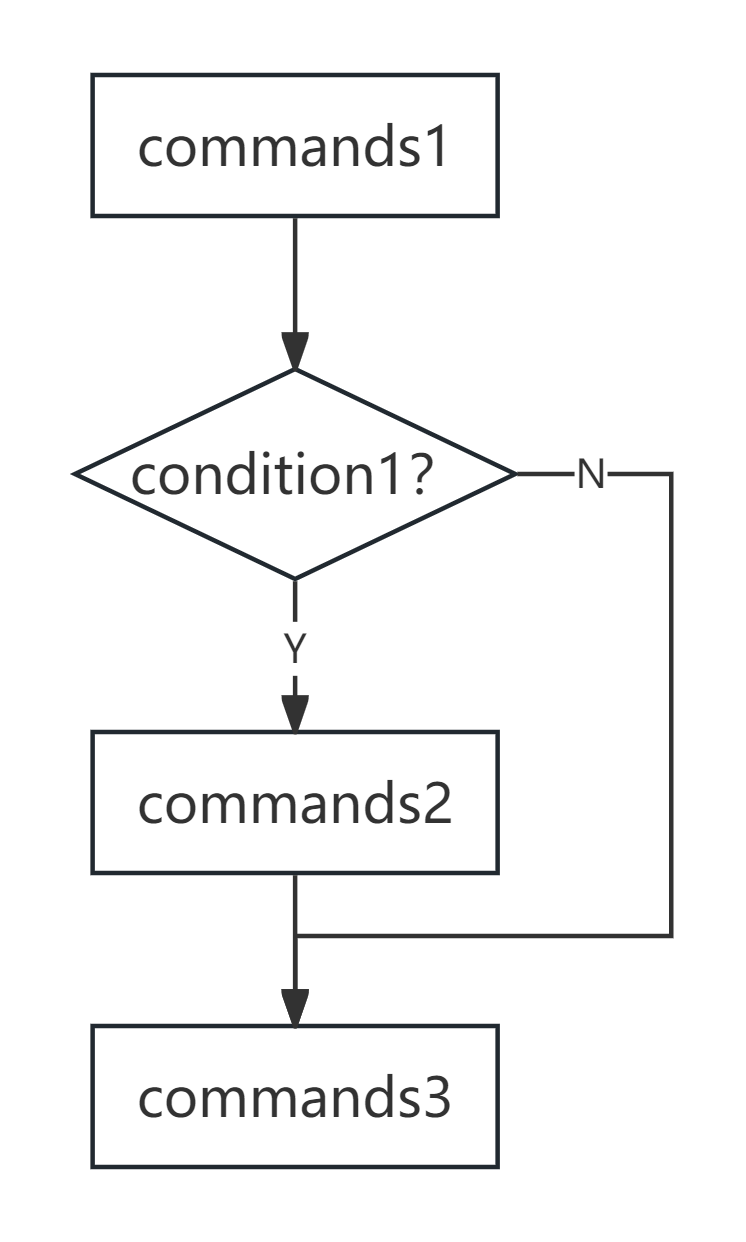
\includegraphics[width=1\linewidth]{Linux基础/Shell脚本基础/判断语句/fig/if语句.png}
    \caption{if语句流程图}
    \label{fig:判断语句-if语句流程图}
\end{figure}

这一段代码当执行完\code{commands1}之后,进行condition判断(条件是否成立),如果(if)成立,然后(then)执行\code{commands2}语句,\emph{否则不执行任何语句},最后执行\code{commands3}。

\begin{attention}
    无论条件是否满足,\code{commands3}都会执行(它是if语句之外的内容,类似于\code{commands1})。在这里的\code{commands1,commands2,commands3}都代表语句(们),每一部分可以是一条或多条语句。\code{condition}是\emph{判断条件},在后面的部分我们将详细介绍如何描述这一部分,简单来说,它描述的内容就是“是否……?”。

    需要特别注意\code{condition}前后与中括号之间的空格,这个空格不能省略!千万不要写成\code{[condition]}这种形式。
\end{attention}

\begin{extend}
    与C语言使用大括号,Python语言使用缩进不同,Shell脚本采用类似于Basic语言和MATLAB那样使用语句表示一整个语句块的方式。一个判断语句一定是以\code{if}开始,以\keyword{fi}结束。这个\code{fi}不代表“finish”或者“final if”等类似含义,而是\code{if}的倒序(在后面其他内容的学习中,会逐渐印证这一点)。

    换言之,在上述代码中,使用缩进与否并不会影响脚本执行效果,但为了增强可读性,我们仍然建议\emph{使用缩进表示每一级之间的层级关系}。事实上,如果你使用\code{vi}创建\code{*.sh}文件时,在输入\code{if}后默认会进行缩进,这也是大多数现代程序语言文本编辑器应当具有的功能。
\end{extend}

\subsection{关系运算符}\label{subsec:判断语句-关系运算符}

任何一个分支判断语句,都应当首先给定一个关系运算,并根据这个结果来判断应该执行哪些命令。在Shell脚本中,我们大致可以将关系运算符分成三类:

\subsubsection{整数比较}

类似于数学上的大于、小于和等于,在Linux当中也有对数值的比较,包括等于(\code{-eq}, \code{==})、不等于(\code{-ne}, \code{!=})、大于(\code{-gt}, \code{>})、小于(\code{-lt}, \code{<})、大于等于(\code{-ge})和小于等于(\code{-le})六种。

\begin{attention}
    在Shell脚本中,许多运算符都是通过上面这种“选项”的形式给出。与一般输入命令类似,选项前后也需要有空格进行分割。

    除了选项格式外,前四种(等于、不等于、大于和小于)我们也给出了类似于C和Python等其他编程语言所使用的运算符格式。这些在Shell脚本中同样可用。但是,对于大于等于和小于等于,没有\code{>=}和\code{<=}。如果你使用了这两个符号,大概率会报错。关于这一问题,目前还没有找到相关的解决方法,如果你有了对应解决方法(当然,不是后面要讲的内容),请联系我。
\end{attention}

\begin{extend}
    这些选项实际上是英文单词的缩写,例如,\code{eq}=equal; \code{ne}=not equal; \code{gt}=greater than; \code{lt}=less than; \code{ge}=Greater or Equal; \code{le}=Less or equal

    在后面你还会见到其他类似的语句,了解它们的实际含义可以帮助你记忆这些选项。
\end{extend}

下面的程序可以用来判断两个数字是否相等(使用前面的\code{if}语句)

\begin{lstlisting}[language=bash,caption=if\_equal,numbers=left]
#!/bin/bash
# 判断两个数字是否相等
a=10
b=10
# if语句判断是否相等
if [ $a -eq $b ]; then
    echo "$a is equal to $b"
fi
# 判断结束后输出
echo "Bye!"
\end{lstlisting}

你可以试着修改变量的值,查看输出结果是否有不同。在上述代码中,当变量相等时,判断结果为“1”,从而执行里面的语句;如果不相等,则判断结果为“0”,跳过里面的语句。无论结果如何,你都会看见第10行所输出的“Bye!”(它在\code{if}语句外面)。

\begin{extend}
    在这里我们提到了“1”和“0”,它们实际上叫做“\emph{布尔值}”或者“\emph{逻辑值}”,也是关系运算(与后面要提到的逻辑运算)的返回结果,其值只包含两种:“真”(也可以用“True”、“1”等代替)和“假”(也可以用“False”、“0”等代替)。
\end{extend}

\begin{attention}
    在中括号里面表示条件判断时,请务必记得中括号内前后要加空格,同时\code{-eq}前后也要加空格。

    在完成\code{if}语句后,不要忘记后面的\code{fi}。
\end{attention}

你也可以试着修改判断条件,例如改成\code{-gt},并修改变量的值,查看结果。

\subsubsection{*浮点数比较}

\begin{extend}
    由于前面所介绍的浮点数在脚本中的局限性,这一部分内容关于浮点数的比较并非必须了解。但如果你确实有此方面需求,在确定不能使用其他如C和Python等编程语言实现的前提下,可以参考这一部分所介绍的方法。

    相比于前面的整数比较,浮点数比较\emph{不能使用}前面的“选项”格式。例如,你写出\code{if [ 3.5 -ne 2.5 ]}是错误的。但是,前面所使用的运算符形式如\code{==, !=}等还是可用的。基于此,对于判断等于和不等于(包括大于和小于),最简单的方法就是使用如\code{if [ 3.5 != 2.5 ]}的格式。

    但是,对于大于等于和小于等于这两种情况,整数部分尚且还有选项可用,浮点数则完全没有对应的简单方法。参考前面\ref{subsec:变量-变量简单运算}一节所介绍的\code{bc}命令,我们可以退而求其次,借助于逻辑运算符的输出结果1和0,来进行判断。例如,我们希望判断3.5是否大于等于2.5,则可以使用\code{if [ \$(echo "3.5 >= 2.5" | bc) -eq 1 ]}这种方式,其中小括号部分借助管道运算符和\code{bc}命令计算\code{3.5 >= 2.5}的结果,根据前面所介绍的逻辑值,输出结果应当是0或1(在这里为1)。然后利用整数的判断方法,判断它与0或1的关系,从而实现浮点数对大于等于和小于等于的判断。
\end{extend}

\subsubsection{字符串判断}

与数值判断类似,字符串也可以进行相应的判断,一般常见的包括判断两个字符串是否相等(\code{==}),是否不相等(\code{!=}),以及判断一个字符串是否为空字符串(\code{-z}和\code{-n})

\begin{attention}
    在判断是否为空字符串时,可以使用\code{-z}和\code{-n},二者在本质上判断的内容是一样的,但返回结果\emph{相反},前者当内容为空时返回“真”,后者当内容不为空时返回“真”。借助于后面的“求非”运算,这二者只需要有一个即可,但为了简洁易读,还是建议在对应的时候使用正确的关系运算符。

    此外,与前面数值判断不同,判断字符串是否为空是“一元运算符”,即\emph{只需要一个变量}。后面的代码则给出了这种一元运算符的一般格式。
\end{attention}

下面的代码实现了判断一个字符串是否为空字符串:

\begin{lstlisting}[language=bash,caption=string\_empty,numbers=left]
#!/bin/bash
# 判断字符串是否为空
read -p "Please input a string:" string
# -n当字符串不为空时为真
if [ -n "$string" ]; then
    echo "Right! I got something ..."
    echo "You input: $string"
fi
echo "Bye!"
\end{lstlisting}

上述代码第5行通过\code{-n}判断输入字符串是否不为空,如果有内容(结果为真),则执行\code{if}语句里面的内容。

\begin{attention}
    在对字符串进行判断时(包括使用二元关系运算符),请务必将字符串变量前后加上双引号。如果不加双引号可能会造成奇怪的错误。
\end{attention}

\subsubsection{文件判断}

Shell脚本也提供了大量的运算符选项,用来判断文件的相关信息。例如,使用\code{-e}判断文件\emph{是否存在},使用\code{-f}(\code{-d})判断是否为普通文件(目录),使用\code{-r, -w, -x}依次判断文件是否可读、可写、可执行。

与前面字符串的代码类似,这里的所有运算符都是一元运算符(即采用\code{<选项> 变量}的格式。例如,下面的代码简单实现了判断文件\code{INCAR}是否存在的功能:

\begin{lstlisting}[language=bash,caption=file\_exist,numbers=left]
#!/bin/bash
# 判断文件INCAR是否存在
if [ -e "INCAR" ]; then
    echo "This file exists."
fi
echo "Bye!"
\end{lstlisting}

其中,\code{-e}后面的\code{"INCAR"}是指当前运行目录下的INCAR文件,你也可以使用绝对路径来描述文件。

\subsection{带有\keyword{else}的判断语句}\label{subsec:判断语句-带有else的判断语句}

下面,我们将进一步介绍\code{if}语句,在之前我们仅仅用来判断某一个条件是否满足,且当满足时执行某一(些)语句。但有时,我们可能有更复杂的需求。例如,判断某一个文件是否存在,如果存在则对文件进行处理,如果不存在则输出文件不存在,并提示用户重新输入。我们姑且忽略到继续输入这一动作(需要用到后面的循环),当条件不满足时如何执行另外的语句?类似于其他编程语言,在Shell当中也可以使用\code{if-else}语句。其基本格式如下:

\begin{lstlisting}[language=bash]
commands1
if [ condition ]; then
    commands2
else
    commands3
fi
commands4
\end{lstlisting}

\begin{figure}
    \centering
    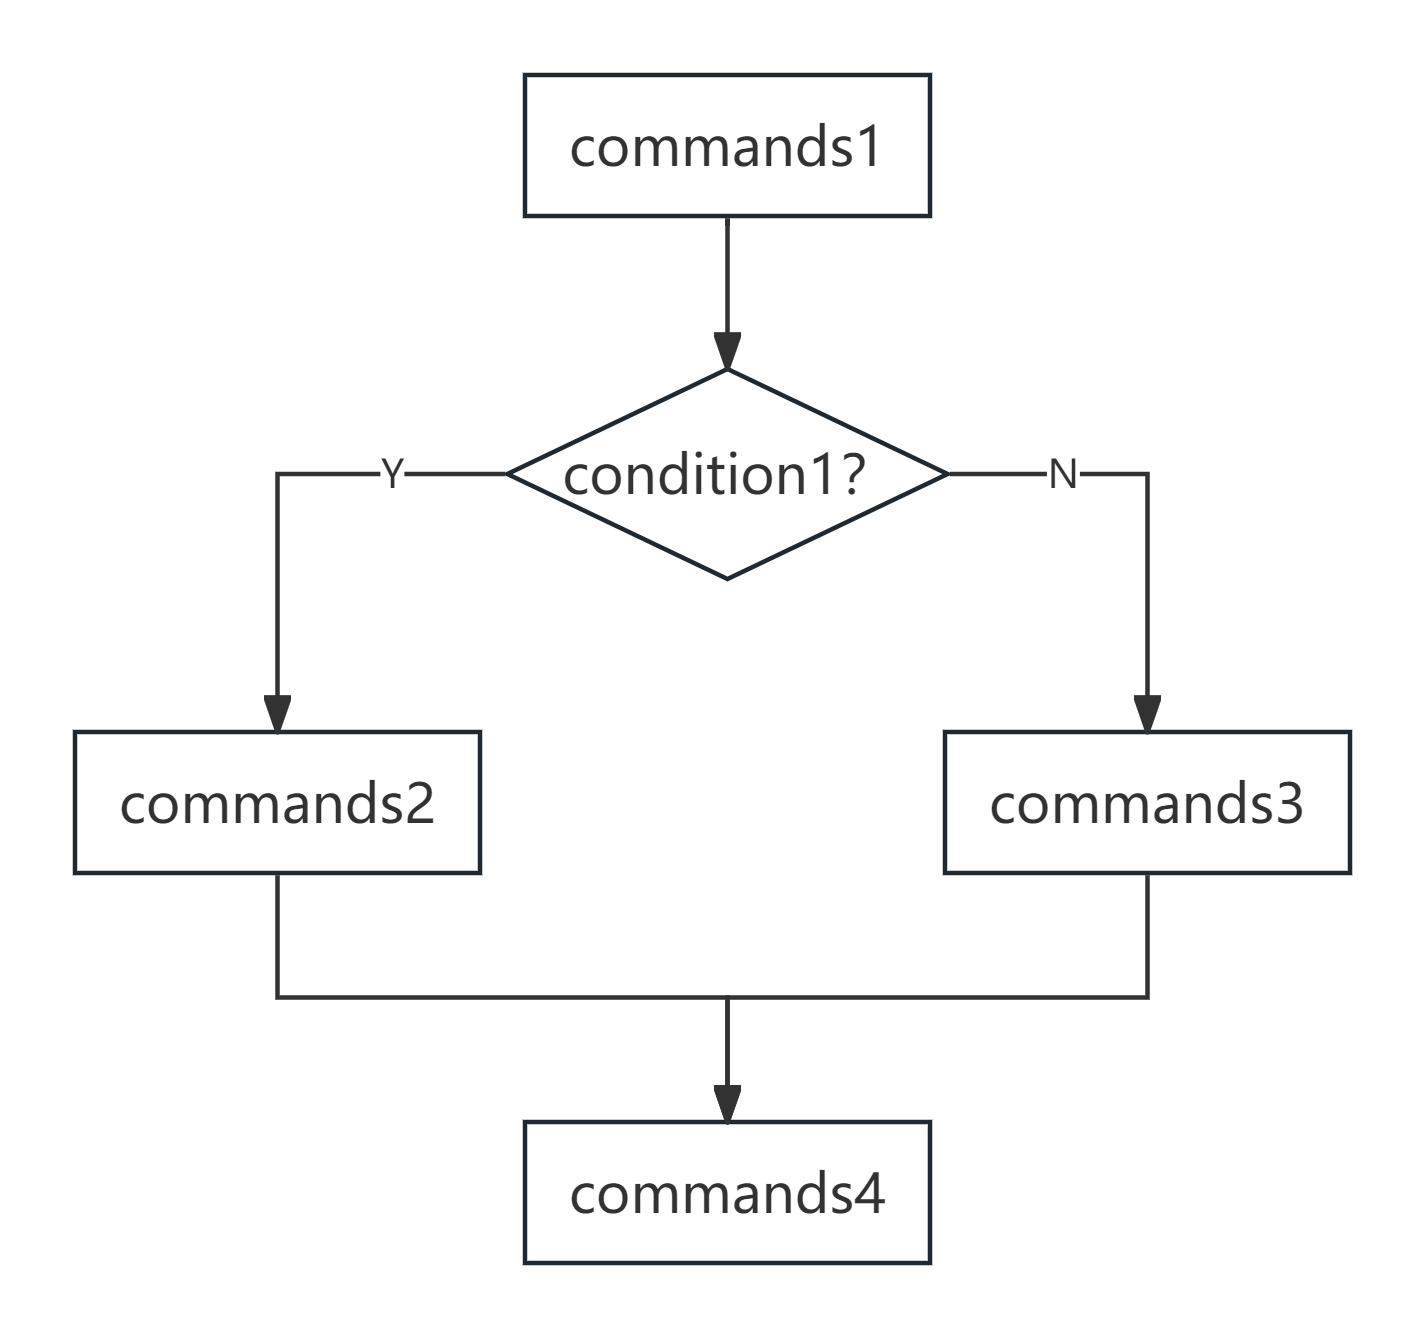
\includegraphics[width=1\linewidth]{Linux基础/Shell脚本基础/判断语句/fig/if-else语句.png}
    \caption{if-else语句}
    \label{fig:判断语句-if-else语句}
\end{figure}

首先程序会执行\code{commands1},然后进行判断,如果(if)条件成立,则(then)执行\code{commands2},否则(else)执行\code{commands3}。 无论结果如何,最后执行\code{commands4}。

下面的代码则是利用上面的语法结构,对前面的判断文件是否存在的脚本(file\_exist)进行了修改:

\begin{lstlisting}[language=bash,caption=file\_exist(2),numbers=left]
#!/bin/bash
# 判断文件INCAR是否存在
if [ -e "INCAR" ]; then
    echo "This file exists."
else
    echo "This file NOT exists."
fi
echo "Bye!"
\end{lstlisting}

除此之外,与Python语言类似,Shell脚本也有\code{if-elif-else}语句,用来对多条件进行判断,语法如下:

\begin{lstlisting}[language=bash]
commands1
if [ condition1 ]; then
    commands2
elif [ condition2 ]; then
    commands3
elif [ condition3 ]; then
    commands4
……
else
    commands5
fi
commands6
\end{lstlisting}

\begin{figure}
    \centering
    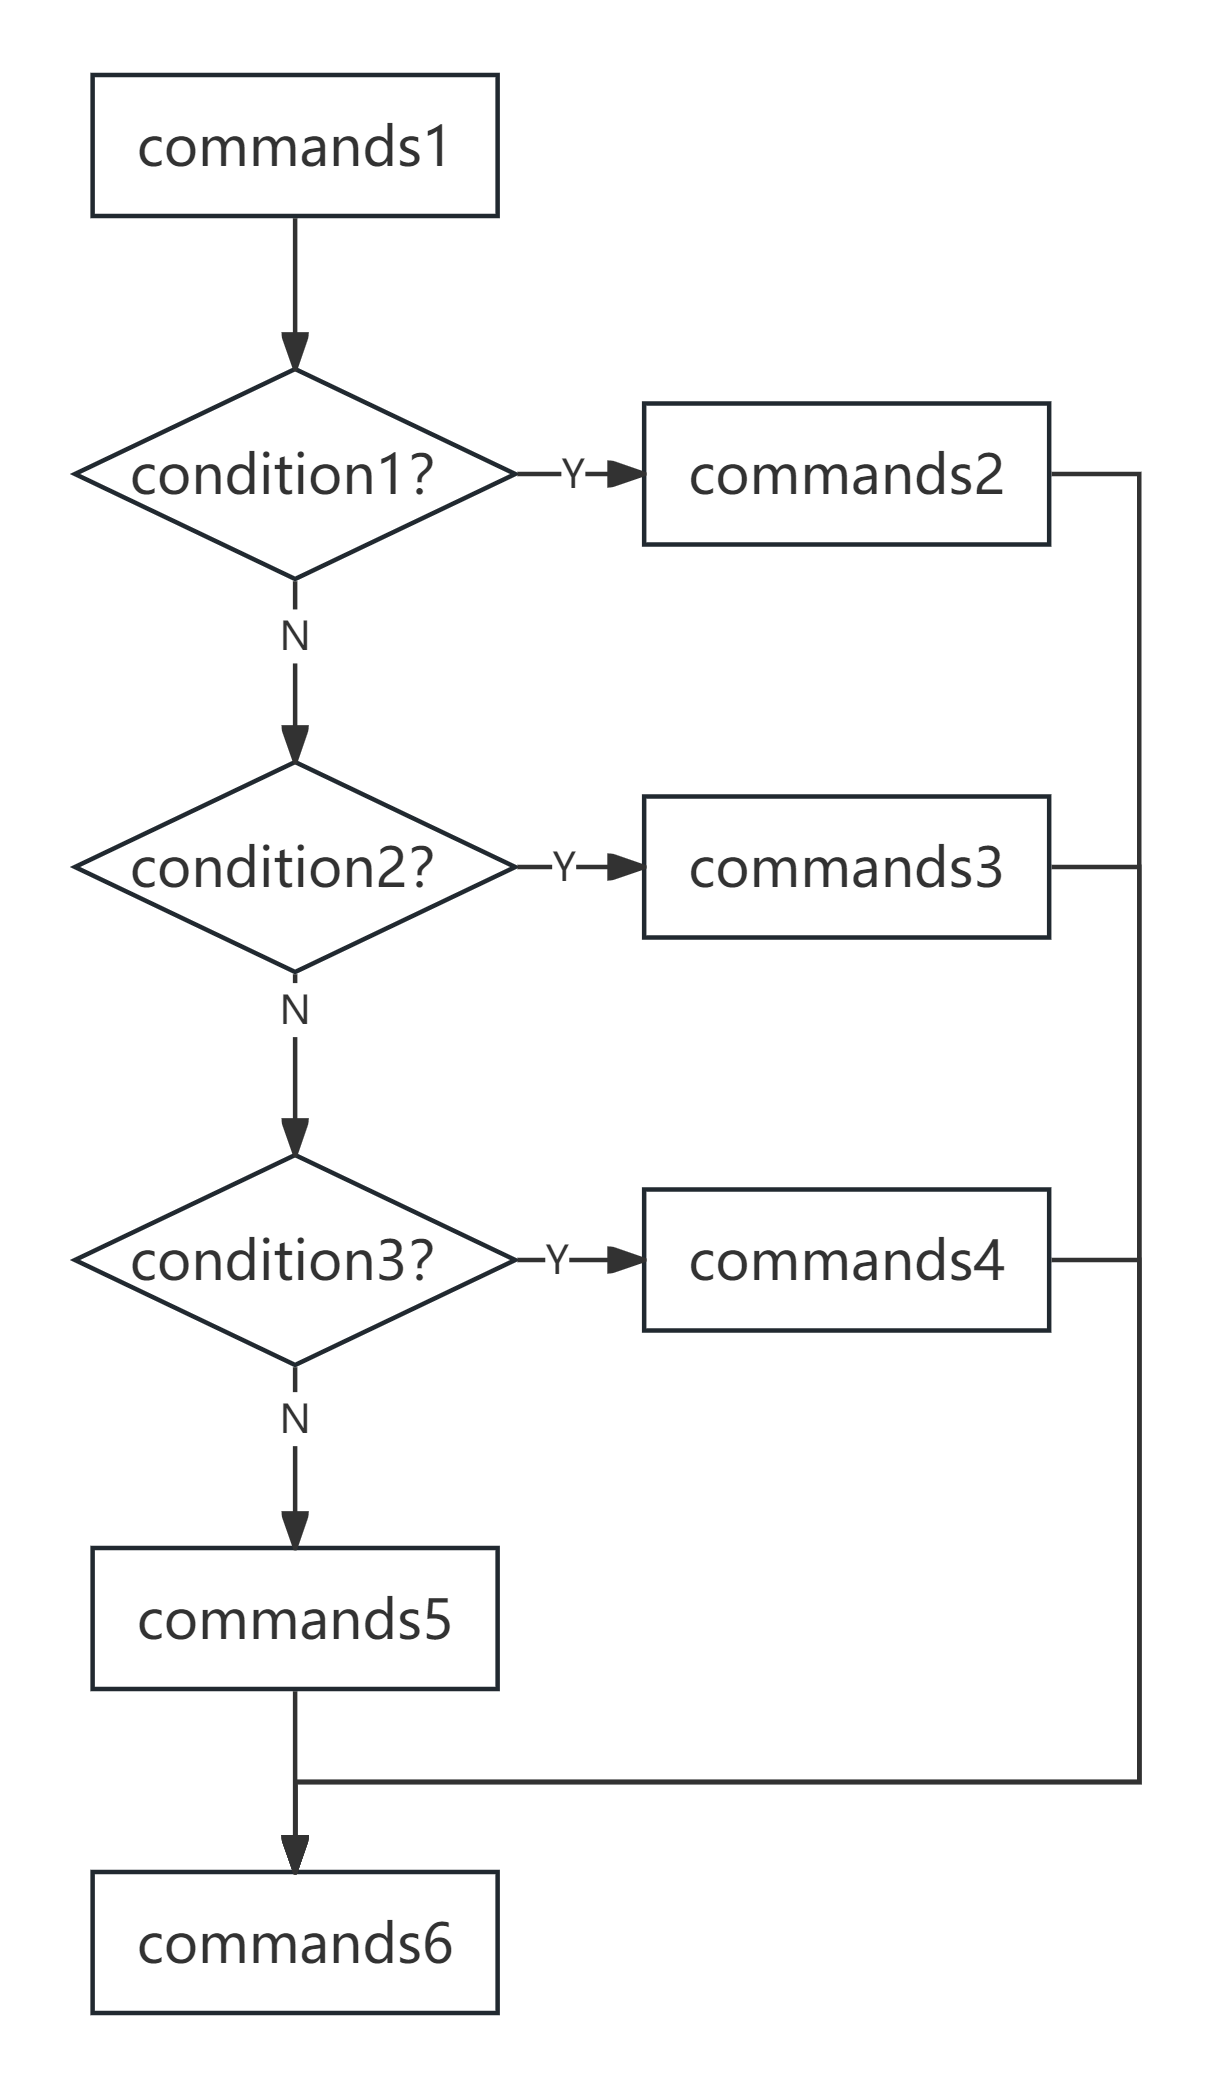
\includegraphics[width=1\linewidth]{Linux基础/Shell脚本基础/判断语句/fig/if-elif-else语句.png}
    \caption{if-elif-else语句}
    \label{fig:if-elif-else语句}
\end{figure}

程序首先判断\code{condition1}是否满足,如果(if)满足,则(then)执行\code{commands2}并结束判断语句,反之如果(else if, elif)满足\code{condition2},则(then)执行\code{commands3}并结束判断语句;反之如果……;否则都不满足(else),执行\code{commands5}。在结束判断语句后,执行\code{commands6}。

下面的程序可以用来判断两个整数之间的关系:

\begin{lstlisting}[language=bash,caption=compare\_number,numbers=left]
#!/bin/bash
# 判断两个整数之间的关系
# 输入两个整数
read -p "Please input an integer(a): " a
read -p "Please input an integer(b): " b
# 判断两个整数之间的关系
if [ $a -eq $b ]; then
    echo "$a = $b"
elif [ $a -gt $b ]; then
    echo "$a > $b"
else
    echo "$a < $b"
fi
echo "Bye!"
\end{lstlisting}

\subsection{嵌套\code{if}语句}\label{subsec:判断语句-嵌套if语句}

与其他编程语言类似,脚本也可以使用嵌套的\code{if}语句,甚至可以更复杂的\code{if-elif-else}嵌套,基于此可以实现复杂的功能。在这里我们不举例子,但有一个需要特别注意的地方:

\begin{attention}
    任何一个\code{if}语句,其后面都需要配合一个\code{fi}作为语句结束。尤其是对于嵌套时的\code{if-else}匹配问题,\code{else}总是与最近的未完成的\code{if}语句匹配(与缩进无关)。例如,下面的代码就违反了第一个原则(\code{if}必须配合有一个\code{fi});同时,看似\code{else}是属于\code{condition1}所对应的判断,但事实上是属于里面的\code{if}。

    \begin{lstlisting}
if [ condition1 ]; then
    commands1
    if [ condition2 ]; then
        commands2
else
    commands3
fi
    \end{lstlisting}

    这段代码是无法正常运行的。所缺少的\code{fi}可以加在\code{commands2}后面,也可以加在\code{commands3}后面,二者所实现的效果是不一样的。你可以尝试一下不同位置所对应的程序运行结果。

\end{attention}

\subsection{逻辑运算}\label{subsec:判断语句-逻辑运算}

在这一节的最后,让我们再来讨论一下逻辑运算。逻辑运算一共分为三种:与(\code{-a})、或(\code{-o})和非(\code{-n})。其中与运算和或运算都是二元运算符,而非运算是一元运算符。

对于与运算而言,\emph{只有当两个值都为真时结果为真}。而对于或运算,\emph{只要有一个为真,结果为真}\footnote{或者还有一种表述是,只有当两个值都为假时,结果为假。}。对于非运算,是一元运算符,其运算结果就是\emph{真变假,假变真}。

下面一个例子实现了判断三个数字是否从小大大排序:

\begin{lstlisting}[language=bash,caption=sort,numbers=left]
#!/bin/bash
# 判断三个数字是否从小到大排序
a=5
b=8
c=10
# 使用与运算符连接
if [ $a -le $b -a $b -le $c ]; then
	echo "$a, $b, $c"
fi
\end{lstlisting}

\begin{extend}
    在这里我们使用多个运算符进行连接,与其他编程语言类似,这里也具有“优先级”的问题。可以简单的理解:关系运算符的优先级高于逻辑运算符的优先级(这在大多数编程语言中都是如此)。虽然上面的写法比较简单,但对于条件复杂的时候可能不具有较好的可读性。因此,可以使用类似于C语言的运算符(\code{\&\&}表示“与”,\code{||}表示“或”),而中间每一个条件使用中括号分割,写作\code{if [ \$a -le \$b ] \&\& [ \$b -le \$c ]}
\end{extend}


\subsection{错误处理}\label{subsec:判断语句-错误处理}
% 请在本节列出可能遇见的错误与解决方法

这一部分有可能出现的错误太多了,以至于难以在这里全部列出。这里仅列举一些常见的错误,且这些错误的解决方法仅是一部分可能的原因。当你出现错误时,请首先查看对应的格式是否正确,并且可以尝试联系我们。

\subsubsection{-bash: <文件名>: line <行号>: syntax error: unexpected end of file}

这是因为在使用\code{if}后没有对应的\code{fi}作为结束。通常出现在嵌套语句中或者一个\code{if}语句太长,到最后忘记了匹配。对此,我们建议,在开始就按照\code{if-fi}对应关系输入。

\subsubsection{bash: [<变量>: command not found...}

这可能是由于你在输入关系表达式时忘记了中括号里前后要加空格。

\subsubsection{-bash: [: missing `]'}
与前面的错误类似,这个通常指右中括号前面没有空格。
% 请在下方的大括号相应位置填写正确的节标题和标签,以及作者姓名
\section{\keyword{case}分支语句}\label{sec:case分支语句}
\sectionAuthor{Jiaqi Z.}

% 请在下方的item内填写本节知识点
\begin{Abstract}
    \item 如何使用\code{case}语句实现分支判断
\end{Abstract}

在前面的\code{if}语句中,已经了解了如何进行判断。理论上了解了\code{if}语句后可以解决所有分支情况,但是有一些情况可能比较特殊。例如,我们希望实现一个菜单界面,此时可能需要用户输入一些指令表示对应的功能。可以想见,如果使用\code{if}语句,将会有许多的判断条件,甚至随着条件的增多,也会影响程序运行效率\footnote{这是因为在进行判断时,脚本需要对所有条件进行遍历。}。

因此,我们希望可以寻找一种方法,直接对变量进行判断,并根据它的值选择合适的语句执行。可以猜到,这就是本节\code{case}语句所要解决的问题。

\subsection{\code{case}语句基本结构}\label{subsec:case分支语句-case语句基本结构}

类似于\code{if}判断语句,\code{case}判断语句的基本结构为:

\begin{lstlisting}[language=bash]
case <变量> in
pattern1)
    statements1
    ;;
pattern2)
    statements2
    ;;
......
*)
    statements3
    ;;
esac
\end{lstlisting}

程序会根据变量所在(in)的模式(可以是一个单独的值,或者正则表达式),选择合适的语句进行执行。例如,如果变量满足\code{pattern1},则会执行\code{statements1}语句;如果满足\code{pattern2},则会执行\code{statements2}语句;以此类推,如果所有的都不满足,则执行\code{*}所对应的\code{statements3}语句。

\begin{attention}
    有几个细节需要特别关注:所有匹配模式都是以小括号作为结束分割(没有左括号);当每一个分支里面的语句结束时,需要有\code{;;}作为结束的标志;在\code{case}语句结束时,需要有\code{esac}作为结束标志。
\end{attention}

\begin{extend}
    正如在\ref{sec:判断语句}中所讲的那样,\code{esac}也是\code{case}的倒序。另外,模式当中的\code{*}实际上可以想见,表示的就是通配符里面的可以表示任意多个字符的\code{*}符号。
\end{extend}

\subsection{\code{case}语句应用}\label{subsec:case分支语句-case分支语句应用}

下面让我们来看几个常见的应用例子。

\subsubsection{单一字符匹配}

在\code{case}语句中,最简单的就是对单独一个字符进行匹配。下面这个例子则实现了一个对菜单的模拟,用户通过输入1或者2来实现对应不同的功能。

\begin{lstlisting}[language=bash,caption=simple\_menu,numbers=left]
#!/bin/bash
# 模拟菜单选项
echo "--------------------"
echo "1) option 1"
echo "2) option 2"
echo "--------------------"
read -p "Please input a number: " number
case $number in
1)
    echo "You input 1"
    echo "I will do something for option 1..."
    ;;
2)
    echo "You input 2"
    echo "I will do something for option 2..."
    ;;
*)
    echo "You did NOT input 1 or 2"
    ;;
esac
echo "Bye!"
\end{lstlisting}

运行上面的代码,可以看见:当用户输入1时,程序可以直接跳转到\code{1)}所对应的语句;对应的,当用户输入2时,可以跳转到\code{2)}所对应的语句;如果输入其他内容(例如输入3),则会跳转到最后提示输入错误。

\begin{attention}
    与\code{if}语句类似,\code{case}语句的前后,即开始的提示和后面的“Bye!”无论哪种情况都会输出,因为它们不属于\code{case}语句内。
\end{attention}

\subsubsection{字符串匹配}

字符串匹配与单一字符匹配完全一样(你可以将单个字符理解成一种特殊的字符串)。但是,在这里我们也有一点新东西要讲。如果我们希望多个选项匹配同一个分支,可以\emph{使用\code{|}符号表示“或”进行分隔}。例如,下面的程序则是根据用户输入的字符串选择特定的分支(有时多个输入对应同一个分支):

\begin{lstlisting}[language=bash,caption=favourite\_band,numbers=left]
#!/bin/bash
# 字符串匹配
read -p "Please input you favourite band: " band
case $band in
"PPP"|"ppp"|"Poppin'Party")
    echo "Thanks! I have known that you like Poppin'Party!"
    ;;
"Roselia"|"R")
    echo "Thanks! I have known that you like Roselia!"
    ;;
"RAS"|"RAISE A SUILEN"|"Raise a suilen")
    echo "Thanks! I have known that you like RAISE A SUILEN!"
    ;;
"MyGO!!!!!"|"mygo"|"mygo!!!!!")
    echo "Thanks! I have known that you like MyGO!!!!!"
    ;;
*)
    echo "Sorry...I don't know this band."
    echo "But now I have known it -- $band"
    echo "Thank you!"
    ;;
esac
echo "Bye!"
\end{lstlisting}

与前面的代码分析完全类似,但特别的是,这里面分支的判断使用\code{|}表示“或”,例如,“PPP”、“ppp”和“Poppin'Party”对应的都是同一个分支;类似地,“R”和“Roselia”也是对应同一个分支,当用户输入“R”或者输入“Roselia”时,得到的结果是一样的。

\subsubsection{正则表达式匹配}

正如一开始所说的那样,在匹配时可以使用\emph{正则表达式}。例如,下面的代码试图读取用户输入的参数为字母还是数字\footnote{为了复习之前的变量种类,我们在这里尝试使用参数给定变量而不是使用\code{read}命令。}:

\begin{lstlisting}[language=bash,caption=number\_or\_letter,numbers=left]
#!/bin/bash
# 读取调用时的选项
export LC_ALL=C
case $1 in
[a-z])
    echo "You input a lowercase"
    ;;
[A-Z])
    echo "You input an uppercase"
    ;;
[1-9])
    echo "You input a number"
    ;;
*)
    echo "You input other things"
    ;;
esac
echo "Bye!"
\end{lstlisting}

\begin{extend}
    也许你足够灵敏,注意到了第3行的\code{export LC\_ALL=C},这句命令表示将程序运行语言环境设置为默认值(可以通过\code{locale}查看环境语言设置),其中\code{C}表示系统默认值。
    
    在这里我们需要添加这一行命令以确保程序运行正确,但这行命令并不影响我们对\code{case}的理解。

    同时,当你运行这一行代码之后,可能程序中的中文注释发生乱码,这并不影响程序运行结果,你可以重新启动系统以恢复开始的状态。
\end{extend}

在调用时,当用户传递给一个小写字母时,则会匹配到\code{[a-z]},相对地,若给定一个大写字母作为参数,则会匹配到\code{[A-Z]}。但是,我们这里只能对用户输入的一个参数进行判断,如果用户输入多个字符的参数(例如\code{abc}),程序则会认为输入了其他内容。如何修改程序呢?请自己思考并尝试写一段代码\footnote{请真的这样做,这会极大提高你的编程思维。},同时自己测试它。(为简单起见,我们只需要匹配第一个字符即可)

同时,正则表达式也可以使用\code{|}作为分隔以进行多个情况的判断,例如,我们希望将上面的代码修改为无论大小写字母都判断为字母,则可以写成下面的样子:

\begin{lstlisting}[language=bash,caption=number\_or\_letter2,numbers=left]
#!/bin/bash
# 读取调用时的选项
export LC_ALL=C
case $1 in
[a-z]|[A-Z])
    echo "You input a letter"
    ;;
[1-9])
    echo "You input a number"
    ;;
*)
    echo "You input other things"
    ;;
esac
echo "Bye!"
\end{lstlisting}


\subsection{错误处理}\label{subsec:分支语句-错误处理}
% 请在本节列出可能遇见的错误与解决方法

\subsubsection{-bash: <文件名>: line <行号>: syntax error near unexpected token `)'}

这可能是因为你在结束分支时少了\code{;;}表示当前分支内结束。如果你了解C语言,你可能会很自然将这这个符号作为C语言中\code{switch-case}的\code{break}语句。但显然,C语言的\code{break}更加灵活(它可以没有从而越过其他分支),但Shell脚本不能没有\code{;;}结束。

\subsubsection{-bash: <文件名>: line <行号>: syntax error near unexpected token `<字符串>'}

这可能是由于你在使用\code{case}语句后忘记结束\code{esac}而后面还有其他语句从而报错。如果后面没有语句,则可能会出现下面的错误:

\subsubsection{-bash: <文件名>: line <行号>: syntax error: unexpected end of file}

这也表明你可能没有使用\code{esac}作为\code{case}语句的结束。
% 请在下方的大括号相应位置填写正确的节标题和标签,以及作者姓名
\section{循环}\label{sec:循环}
\sectionAuthor{Jiaqi Z.}

% 请在下方的item内填写本节知识点
\begin{Abstract}
    \item 如何使用\code{for}循环
    \item 如何使用\code{while}循环
    \item 如何使用\code{until}循环
    \item \code{while}循环和\code{until}循环的区别
\end{Abstract}

在前面介绍高级Linux命令时,我们曾说过脚本处理的任务大多是\emph{批量处理}任务,而批量处理的一个基本方法就是使用循环语句(毕竟没有人会想写上上百行相同的代码)。在\ref{sec:简单for循环}一节中,我们介绍过\code{for}循环的使用,当时是在命令行中编写的。本节我们将首先复习一下\code{for}循环的基本使用方法,以及它在脚本程序中的格式(和命令行类似),然后再介绍两种不同的循环语句——\code{while}循环和\code{until}循环——它们虽然在一定程度上是等价的,但在不同的情况下,选择合适的循环语句会让程序更加简洁易读。

\subsection{\code{for}循环}\label{subsec:循环-for循环}

下面的代码完整演示了常见的三种\code{for}循环格式:

\begin{lstlisting}[language=bash,numbers=left,caption={for\_example}]
#!/bin/bash
# 使用for循环输出
# 简单列表
for i in 1 2
do
    echo $i
done
echo ""
# 生成列表
for i in $(seq 1 2 10)
do
    echo $i
done
echo ""
# 使用C语言格式
for ((i=0;i<10;i++))
do
    echo $i
done
\end{lstlisting}

其中第8行、第14行使用\code{echo ""}输出一个空行用来区分不同的输出结果。

\subsubsection{简单列表}

使用基本列表的格式调用\code{for}循环的基本格式为:

\begin{lstlisting}[language=bash]
for <变量名> in <列表>
do
    循环体
done
\end{lstlisting}

\begin{extend}
    在循环语句内部的语句,我们常常称其为\emph{循环体}(实际上和前面所说的\code{commands},程序块,语句块等一样)
\end{extend}

在这里的\code{<列表>}可以如同上面的代码一样直接以空格分隔表示,也可以与\ref{sec:简单for循环}一节所说的那样使用大括号将其括起来,并用逗号分割。

\begin{attention}
    一个常见的错误是将两者混淆,即\emph{使用大括号表示列表的同时,其内部元素用空格分隔}。可以验证的是,这并不会如你所愿得到正确的信息。事实上,空格的“优先级”会高于大括号的“优先级”(这里加引号表示这不是传统意义上运算符的优先级),当括号和空格同时存在时,程序会将列表解析为\emph{以空格分隔的列表},从而在输出的前后(第一个元素和最后一个元素)带有大括号。
\end{attention}

与前面的介绍类似,在循环体内使用变量需要加\code{\$}符号。

\subsubsection{生成列表}

与\ref{sec:简单for循环}里所介绍的方法类似,可以使用\code{seq}命令生成序列。与前面所介绍的方法不同的是,前面所使用的是\code{`}符号括起来的命令,而在脚本中,由于将\code{seq}看作是一个命令,因此与前面\ref{subsec:输入-读取命令作为输入}一节所介绍的输入方式类似,使用\code{\$()}的方式得到\code{seq}命令的结果,并将其作为一个变量传递给\code{for}循环。

当然,也可以使用前面所说的\code{..}的方式生成序列。但需要复习的是:对于\code{seq}语句而言,三个参数分别是\emph{开始、步长、结束};而对\code{..}方式而言,三个参数分别是\emph{开始、结束、步长}。因此,上面代码的\code{seq 1 2 10}也可以写作\code{\{1..10..2\}}

\subsubsection{运算格式生成}

如果你熟悉C语言的话,这一种格式会显得很“亲切”。因为它的基本结构与C语言几乎完全类似,类似地写法,如果让我们用C语言实现上面代码的第3部分,则可以写作这样:

\begin{lstlisting}[language=C,numbers=left]
#include <stdio.h>
void main()
{
    for (int i=0;i<10;i++)
        printf("%d\n",i);
}
\end{lstlisting}

可以看到,相比于C语言,脚本只是一个括号和两个括号的区别\footnote{由于C语言是强类型语言,因此在for循环条件中定义了变量类型\code{int},但这不是必需的,因为完全可以将变量定义放在循环外面作为单独的语句,此时C语言的括号内与脚本的括号内就完全相同了。在比较二者不同时,我们有意忽略了这一点,只是为了让大家关注到本质}。

\begin{attention}
    在脚本的\code{for}循环当中,括号前面没有\code{\$}符号,也千万不要“画蛇添足”加上这个符号。
\end{attention}



\subsection{\code{while}循环}\label{subsec:循环-while循环}

与C语言的\code{while}循环类似,在bash脚本中也存在根据条件判断循环与否的\code{while}循环。其基本格式如下:

\begin{lstlisting}[language=bash]
while [ condition ]
do
    循环体
done
\end{lstlisting}

其中,\code{condition}表示\emph{循环进行的条件},其格式与\ref{sec:判断语句}当中所介绍的条件表达式类似。例如,下面的代码实现了从0到9的输出

\begin{lstlisting}[language=bash,numbers=left,caption={while\_example}]
#!/bin/bash
# 使用while循环输出数字
i=0
while [ $i -lt 10 ]
do
    echo $i
    ((i++))
done
\end{lstlisting}

可以复习一下,条件\code{-lt}表示\emph{小于},因此,循环体进行的条件是\emph{变量\code{i}小于10}。当条件满足时,程序进行循环体(\code{do}和\code{done}中间的部分)。因此,程序会从0开始,逐渐输出并加1,直到条件不满足时(\code{i}为10)则停止循环。

\begin{attention}
    与\code{for}循环相比,\code{while}循环更有可能写出“死循环”语句。所谓“死循环”,指的是程序在循环体内一直循环,永无停止。在上面的代码中,如果少了那句\code{((i++))},则变量始终为0,条件始终满足,从而无法停止。

    具体的解决方法,可以见下一节所介绍的\code{break}和\code{continue}语句。
\end{attention}

此外,在上面程序的第7行,使用\code{((i++))}表示进行计算,这是比较简洁的C风格递增运算符,类似的还有递减运算符\code{--}。这种方式的使用需要以两个括号括起来。你也可以使用\ref{sec:变量}一节所介绍的方法,使用\code{i=\$(( \$i + 1 ))}的方式。这二者在这一功能上是等价的。

\subsection{\code{until}循环}\label{subsec:循环-until循环}

与\code{while}循环几乎完全类似,bash脚本中\code{until}循环的格式为:

\begin{lstlisting}[language=bash]
until [ condition ]
do
    循环体
done
\end{lstlisting}

与上面的\code{while}循环格式比较可以发现,除了关键字从\code{while}变成了\code{until}外,其他语句在格式上没有任何不同。但\code{until}循环的最大特点是:\emph{循环体执行的条件是\code{condition}为假},即你可以简单的将其理解为:循环体会一直执行,“直到”(until)条件为真。

\begin{attention}
    这一点稍微有点绕,但上面的两种表述是“等价”的。对\code{while}循环而言,当条件为真时执行循环体,而对\code{until}循环而言,当条件为真时退出循环(当条件为假时进入循环)
\end{attention}

\begin{extend}
    在C语言中,确实没有类似的循环与其对应,但我们可以从其他一些编程语言中找到这个例子,一个最简单的例子就是——Visual Basic语言(简称VB语言)。在VB语言中,也存在类似的\code{until}循环,其格式为:

    \begin{lstlisting}
Do 
    循环体
Loop Until 条件
    \end{lstlisting}

    如果你熟悉VB语言的话,bash脚本的\code{until}循环与VB语言的\code{until}循环最大的不同在于\emph{VB语言的条件是放在循环后面(类似于C语言的\code{do-while}循环)}

    当然,如果你不熟悉VB语言的话,也不必担心。这一部分仅仅是对那些熟悉VB语言的读者所准备的,以防他们混淆条件的位置。如果你本来不了解VB语言的话,这一部分完全可以跳过。
\end{extend}

可以简单想见的是,\code{while}循环和\code{until}循环之间的转换仅仅是“\emph{条件的取反}”,例如,上面关于\code{while}循环的例子,我们只需要将里面的条件\code{\$i -lt 10}改为\code{\$i -ge 10},同时将\code{while}改为\code{until}就可以实现相同的功能。这一部分代码我们不做演示,请自己尝试修改上面的代码并测试其输出结果是否与之前的结果一致。



% \subsection{错误处理}\label{subsec:节标题-错误处理}
% % 请在本节列出可能遇见的错误与解决方法

% \subsubsection{错误1}

% \subsubsection{错误2}

% \subsubsection{错误3}
% 请在下方的大括号相应位置填写正确的节标题和标签,以及作者姓名
\section{循环控制}\label{sec:循环控制}
\sectionAuthor{Jiaqi Z.}

% 请在下方的item内填写本节知识点
\begin{Abstract}
    \item 如何使用\code{break}语句
    \item 如何使用\code{continue}语句
\end{Abstract}

在\ref{sec:循环}一节中,我们曾简单提到了“死循环”问题。在当时看来,死循环是一个应当避免的“错误”,但事实可能不总是如此——在有些情况下,我们可能不得不希望使用死循环。例如,我们希望一直读取用户的输入,直到用户输入0时退出。此时当然可以使用\code{while}循环或者\code{until}循环来解决这一问题。但还有一种思路——设计一个死循环,当用户输入0时跳出循环。

\begin{extend}
    在其他领域,死循环可能是更常见的。例如,在一些单片机系统中,会使用死循环来执行对应的任务,例如读取传感器数据、显示处理数据等;而在Windows操作系统中,任何一个窗口在创建时都会启动叫做“消息循环”的死循环来保持窗口——对于Windows来说,如果没有这个死循环,窗口会立即关闭。

    因此,在程序中,死循环并不是“绝对的错误”,而要根据需要选择。一些可控的、必需的死循环也是程序所必要的一部分。
\end{extend}

回到最开始的例子,在bash语言中,我们有两种方式对循环语句进行控制——\code{break}语句和\code{continue}语句。其中前者表示“终止循环”,而后者表示“继续循环”



\subsection{使用\code{break}停止循环}\label{subsec:循环控制-使用break停止循环}

\begin{extend}
    本节所要介绍的\code{break}与\code{continue},在使用方式与效果上与C语言的\code{break}和\code{continue}\emph{完全相同}。因此,如果你足够熟悉C语言,本节完全可以跳过。但我们还是建议你通过阅读这一节复习一下相关的内容。
\end{extend}

\code{break}语句的作用是用来\emph{跳出循环},例如,下面的程序,用户输入一系列数字,当用户输入0时,循环结束,输出“end”

\begin{lstlisting}[language=bash,numbers=left,caption={break\_example}]
#!/bin/bash
# break跳出循环
read a
while [ true ]
do
    if [ $a -eq 0 ]; then
        break
    fi
    echo $a
    read a
done
echo "end"
\end{lstlisting}

在第4行,我们设置了一个条件\code{true},使循环条件始终成立,从而令其成为一个“死循环”。在第6行利用\code{if}语句判断输入的变量是否为0,如果是0,则通过\code{break}跳出循环,执行最后一行的“end”输出。如果输入的数字不为0,则输出对应的变量值。

\begin{attention}
    请务必仔细思考一下,程序的第10行又写了一句\code{read a}有什么作用?如果没有这句命令会发生什么?在程序中有两句\code{read}命令稍显繁琐,有没有简单的方法使用一句即可实现相同的功能?
\end{attention}

除了在\code{while}循环外,\code{for}循环和\code{until}循环也可以使用\code{break}语句。例如,下面的程序遍历了10-20之间所有的数字,且当数字为7的倍数时停止。

\begin{lstlisting}[language=bash,numbers=left,caption={break\_example2}]
#!/bin/bash
# 在for循环中使用break语句
# 当遍历到7的倍数时停止
for i in {10..20}
do
    if [ $(( $i%7 )) -eq 0 ]; then
        break
    fi
    echo $i
done
echo "end" 
\end{lstlisting}

其中,变量\code{i}会依次从10递增到20,当\code{i}取值为14时,满足7的倍数\footnote{这里使用常见的方法——“取余”判断倍数,具体的计算方法可以查看\ref{subsec:变量-变量简单运算}一节。},从而进入条件判断内,执行\code{break}命令,跳出循环输出\code{end}

\begin{attention}
    上面的两个例子还说明了,\code{break}跳出循环是“立刻跳出”,即如果循环体内有剩下的其他语句也不会执行了。例如,上面的判断倍数的例子,当\code{i}取值为14时,也没有输出这个值(因为输出命令在\code{break}后面。

    可以尝试一下:如果将\code{echo \$i}放在循环体内第一行,输出结果会有什么不同?
\end{attention}

\subsection{使用\code{continue}跳过循环}\label{subsec:循环控制-使用continue跳过循环}

与C语言类似,在bash脚本中,也可以使用\code{continue}跳过循环。这里所说的“跳过”,指的是\emph{跳过当前轮次的循环}。让我们直接来看一个例子——假设将上面判断7的倍数的例子中的\code{break}改成\code{continue},看看会发生什么。

\begin{lstlisting}[language=bash,numbers=left,caption={continue\_example2}]
#!/bin/bash
# 使用continue语句跳过循环
for i in {10..20}
do
    if [ $(( $i%7 )) -eq 0 ]; then
        continue
    fi
    echo $i
done
echo "end" 
\end{lstlisting}

运行后可以看见,程序输出了10-20的所有数字,除了14。这是因为当变量\code{i}为14时,条件满足,执行\code{continue}语句,跳过了当前轮次的循环,直接进入下一个循环轮。与\code{break}类似,这里也不再执行后面的语句(即不会输出14这个数字)

虽然\code{continue}在语法上和\code{break}类似,难度也不大,但其使用时存在一个非常潜在的“隐患”。让我们再来看一下本节最开始的程序,如果将其中的\code{break}改成\code{continue},会发生什么?此时代码长成下面这样:

\begin{lstlisting}[language=bash,numbers=left,caption={continue\_example}]
#!/bin/bash
# 使用continue跳过0的判断,继续输入?
read a
while [ true ]
do
    if [ $a -eq 0 ]; then
        continue
    fi
    echo $a
    read a
done
echo "end"
\end{lstlisting}

一些“粗心大意”的人可能会认为:这段代码一直读取用户的输入并输出对应的内容,当用户输入0时跳过输出。让我们执行一下这段代码,当用户输入非0的数字时,程序很正常地输出对应的数字;当用户输入0时,程序也确实跳过了0的输出;但是,\emph{从这开始程序再也读取不了输入了}。从程序代码的执行过程可以很容易理解这一点,当用户输入0时,此时变量\code{a}的值为0,进入条件判断内,跳过当前循环。正如前面所说的那样,程序跳过循环\emph{不再执行后面的语句}。因此,在后面的循环中变量\code{a}始终保持0的值,即始终在4-7行语句间循环。

\begin{attention}
    对于\code{for}循环而言,由于它是对序列进行遍历,一般情况下总是“有限”的,因此循环总是能停止的。而对于\code{while}和\code{until}循环而言,在循环开始和\code{continue}中间,\emph{要有改变循环条件或者终止循环的语句},否则循环将陷入“死循环”。
\end{attention}


% \subsection{错误处理}\label{subsec:节标题-错误处理}
% % 请在本节列出可能遇见的错误与解决方法

% \subsubsection{错误1}

% \subsubsection{错误2}

% \subsubsection{错误3}